\documentclass[12pt,fleqn]{report} 
\usepackage[top=2cm,bottom=2cm,left=2cm,right=2cm,headsep=10pt,letterpaper]{geometry}
\usepackage[utf8]{inputenc}
\usepackage{amsmath}
\usepackage{amssymb}
\usepackage{amsthm}
\usepackage{graphicx}
\usepackage{enumitem}
\usepackage{pdfpages}
\renewcommand{\familydefault}{\sfdefault}
\newtheorem{esempio}{Esempio}

\title{Appunti di Fisica}
\author{Elisa Solinas}
\date{Aggiornato il \today}

\begin{document}

\maketitle
\tableofcontents

\chapter{Meccanica}

\section{Calcolo vettoriale}
Consideriamo due vettori in un sistema di coordinate $(xyz)$:
\begin{displaymath}\begin{aligned}
	\vec{a} = (a_1, a_2, a_3)\\
    \vec{b} = (b_1, b_2, b_3)    
\end{aligned}\end{displaymath}
\begin{figure}[h!]
       	\centering
        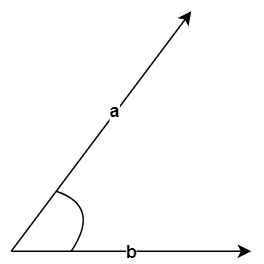
\includegraphics[scale = 0.4]{Pictures/vettori.png}
    \end{figure}
    
\subsection{Modulo di un vettore}
\begin{displaymath}\begin{aligned}
	|\vec{a}| = \sqrt{a_1^2 + a_2^2 + a_3^2}
\end{aligned}\end{displaymath}

\subsection{Somma di due vettori}
\begin{displaymath}\begin{aligned}
	\vec{a} + \vec{b} = (a_1 + b_1, a_2 + b_2, a_3 + b_3)
\end{aligned}\end{displaymath}

\subsection{Differenza di due vettori}
\begin{displaymath}\begin{aligned}
	\vec{a} - \vec{b} = (a_1 - b_1, a_2 - b_2, a_3 - b_3)
\end{aligned}\end{displaymath}

\subsection{Prodotto scalare di due vettori}
\begin{displaymath}\begin{aligned}
	\vec{a} \cdot \vec{b} = (a_1 \cdot b_1) + (a_2 \cdot b_2) + (a_3 \cdot b_3) = |a| \cdot |b| \cdot \cos{\theta}
\end{aligned}\end{displaymath}
\subsubsection{Osservazioni}
\begin{itemize}
   	\item{Il prodotto scalare di due vettori perpendicolari è nullo.}
\end{itemize}

\subsection{Prodotto vettoriale di due vettori}
Il prodotto vettoriale tra due vettori è perpendicolare a entrambi.
\begin{displaymath}
   	\vec{a} \times \vec{b} = 
    \begin{bmatrix}
   		\vec{i} & \vec{j} & \vec{k}\\
       	a_1 & a_2 & a_3 \\
       	b_1 & b_2 & b_3
   	\end{bmatrix} =
    (a_2 \cdot b_3 - a_3 \cdot b_2) \cdot \vec{i}
    - (a_1 \cdot b_3 - a_3 \cdot b_2) \cdot \vec{j}
    + (a_1 \cdot b_2 - a_2 \cdot b_1) \cdot \vec{k}
\end{displaymath}

\subsubsection{Osservazioni}
\begin{itemize}
\item{Il prodotto vettoriale di due vettori è perpendicolare a entrambi.}
\item{Il prodotto vettoriale di due vettori è anticommutativo, cioe:
   	\begin{displaymath}
       	\vec{a} \times \vec{b} = - \vec{b} \times \vec{a}
    \end{displaymath}}
\item{Il prodotto vettoriale di due vettori paralleli è nullo. } 
\item{I versori della base canonica ($\vec{i}, \vec{j}, \vec{k}$) soddisano le seguenti equazioni:
	\begin{displaymath}\begin{aligned}
		\vec{i} \times \vec{j} = \vec{k} \\
		\vec{i} \times \vec{k} = - \vec{j} \\
		\vec{j} \times \vec{k} = \vec{i}
	\end{aligned}\end{displaymath}}
\end{itemize}

\subsection{Calcolo di un vettore che collega due punti}
\begin{displaymath}\begin{aligned}
   	A = (a_1, a_2) \qquad B = (b_1, b_2)\\
    \vec{AB} = (b_1 - a_1, b_2 - a_2)
\end{aligned}\end{displaymath}

\section{Equazioni del moto}
\subsection{Moto rettilineo uniforme}
\begin{displaymath}\begin{aligned}
	v = \frac{\Delta s}{\Delta t}\\
    s = s_0 + v \cdot t\\
\end{aligned}\end{displaymath}
\subsection{Moto rettilineo uniformemente accelerato}
\begin{displaymath}\begin{aligned}
    a = \frac{\Delta \vec{v}}{\Delta t}\\
    v = v_0 + a \cdot t\\
    x = x_0 + v_0 \cdot t + \frac{1}{2} a\cdot t^2\\
    v^2 = v_0^2 +2a(x-x_0)
\end{aligned}\end{displaymath}

\subsection{Moto circolare uniforme}
Nel moto circolare uniforme, il vettore velocità $\vec{v}$ ha solo componente tangente alla circonferenza:
\begin{displaymath}\begin{aligned}
    \vec{v} = \vec{\omega} \times \vec{r}\\
    \vec{a} = \frac{v^2}{r^2} \cdot \vec{r} = \omega^2 \cdot \vec{r} 
\end{aligned}\end{displaymath}	

\section{Leggi di Newton}
\subsection{Prima legge di Newton}
Un corpo mantiene il proprio stato di quiete o di moto rettilineo uniforme, finché una forza non agisce su di esso.

\subsection{Seconda legge di Newton}
L'accelerazione di un corpo è direttamente proporzionale e ha la stessa direzione della forza netta agente su di esso, mentre invece è inversamente proporzionale alla sua massa
\begin{displaymath}
	\vec{F} = m \cdot \vec{a}
\end{displaymath}

\subsection{Terza legge di Newton}
Se un corpo $A$ esercita una forza $\vec{F}_{AB}$ su un corpo $B$, allora il corpo $B$ esercita sul corpo $A$ una forza $\vec{F}_{BA}$
\begin{displaymath}
  	\vec{F}_{AB} = -\vec{F}_{BA}
\end{displaymath}

\begin{esempio}
  	La forza $\vec{F}_{12}$ esercitata da $q_1$ su $q_2$ è uguale in modulo e opposta in direzione alla forza $\vec{F}_{21}$ esercitata da $q_2$ su $q_1$.
 	\begin{displaymath}
         	|\vec{F}_{12}| = |\vec{F}_{21}| = k_e \cdot \frac{q_1 \cdot q_2}{r^2}
	\end{displaymath}
   	Nel caso in cui le due cariche abbiano lo stesso segno:
    	\begin{figure}[h!]
			\centering
        	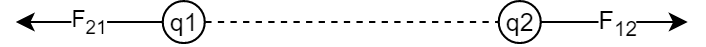
\includegraphics[scale=0.4]{Pictures/esempio1.png}
		\end{figure}
    	\begin{displaymath}
    		\vec{F}_{12} = - k_e \cdot \frac{q_1 \cdot q_2}{r^2} \cdot \vec{u}_r\\
\vec{F}_{21} = k_e \cdot \frac{q_1 \cdot q_2}{r^2} \cdot \vec{u}_r
    	\end{displaymath}
Nel caso in cui le due cariche abbiano segno opposto:
    	\begin{figure}[h!]
			\centering
        	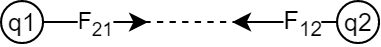
\includegraphics[scale=0.4]{Pictures/esempio2.png}
		\end{figure}
    	\begin{displaymath}
    		\vec{F}_{12} = k_e \cdot \frac{q_1 \cdot q_2}{r^2} \cdot \vec{u}_r\\
\vec{F}_{21} = - k_e \cdot \frac{q_1 \cdot q_2}{r^2} \cdot \vec{u}_r
    	\end{displaymath}
\end{esempio}

\chapter{Elettrostatica}

\section{Legge di Coulomb}
  
La forza $\vec{F}_{12}$ esercitata da $q_1$ su $q_2$ è uguale in modulo e opposta in direzione alla forza $\vec{F}_{21}$ esercitata da $q_2$ su $q_1$.
    \begin{displaymath}
    	|\vec{F}_{12}| = |\vec{F}_{21}| = k_e \cdot \frac{q_1 \cdot q_2}{r^2}
    \end{displaymath}
Nel caso in cui le due cariche abbiano lo stesso segno:
	\begin{figure}[h!]
      \centering
      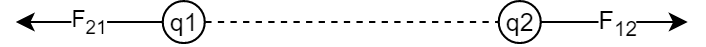
\includegraphics[scale=0.4]{Pictures/esempio1}
  \end{figure}
  	\begin{displaymath}\begin{aligned}
    	\vec{F}_{12} = - k_e \cdot \frac{q_1 \cdot q_2}{r^2} \cdot \vec{u}_r\\
        \vec{F}_{21} = k_e \cdot \frac{q_1 \cdot q_2}{r^2} \cdot \vec{u}_r
    \end{aligned}\end{displaymath}
Nel caso in cui le due cariche abbiano segno opposto:
    \begin{figure}[h!]
    	\centering
        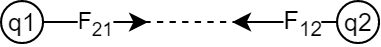
\includegraphics[scale=0.4]{Pictures/esempio2.png}
	\end{figure}
    \begin{displaymath}\begin{aligned}
        \vec{F}_{12} = k_e \cdot \frac{q_1 \cdot q_2}{r^2} \cdot \vec{u}_r\\
        \vec{F}_{21} = - k_e \cdot \frac{q_1 \cdot q_2}{r^2} \cdot \vec{u}_r
    \end{aligned}\end{displaymath}
    
\section{Principio di sovrapposizione}
In un sistema di $n$ cariche, volendo valutare la forza totale agente su una carica $q$, è necessario sommare le forze esercitate da ciascuna carica. Ciascuna di queste forze agisce come se fosse l'unica presente.
	\begin{displaymath}\begin{aligned}
		\vec{F} = \sum_{i=1}^n k_e \cdot \frac{q \cdot q_i}{r_i^2} \cdot \vec{u}_{r_i}
	\end{aligned}\end{displaymath}

\section{Campo elettrico}
Dato un sistema di $n$ cariche, su una carica di prova $q$, agisce un campo elettrico $\vec{E}$ dato da:
	\begin{displaymath}\begin{aligned}
		\vec{E} = \sum_{i=0}^n k_e \cdot \frac{q_i}{r_i^2}\vec{u}_{r_i}
	\end{aligned}\end{displaymath}
La forza agente su $q$ può essere espressa come:
	\begin{displaymath}
		\vec{F} = q \cdot \vec{E}
	\end{displaymath}
    
\section{Teorema di Gauss per il campo elettrico}
Il teorema di Gauss per il campo elettrico permette di calcolare il flusso del campo elettrico generato da una certa distribuzione di carica elettrica attraverso una superficie senza svolgere i calcoli prescritti dalla definizione di flusso.
Data una superficie chiusa $S$ contenente $n$ cariche elettriche (positive o negative), il flusso del campo elettrico (generato dalle cariche) attraverso tale superficie è uguale al rapporto tra carica totale contenuta nella superficie chiusa e la costante dielettrica $\epsilon$ del mezzo in cui si trovano le cariche ($\epsilon_0$ nel vuoto):
\begin{displaymath}
	\Phi_S(\vec{E}) = \frac{\sum_{i=1}^n q_i}{\epsilon_0}
\end{displaymath}

\subsection{Distribuzione lineare}
    \begin{figure}[h!]
    	\centering
    	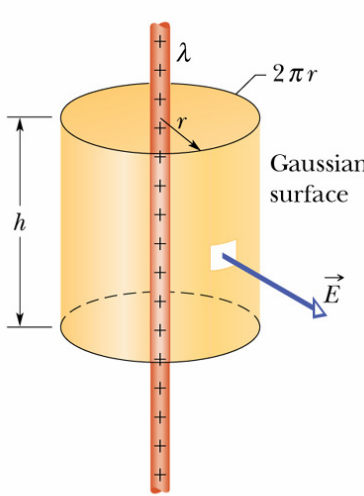
\includegraphics[scale=0.4]{Pictures/esempio3.png}
    \end{figure}
Il campo elettrico $\vec{E}$ è perpendicolare alla superficie gaussiana:
	\begin{itemize}
    	\item{$\Phi(\vec{E})$ attraverso le basi è nullo.}
        \item{$\Phi(\vec{E})$ attraverso la superficie laterale è pari a $E \cdot (2 \cdot \pi \cdot r \cdot h)$.}
    \end{itemize}
Per il teorema di Gauss:
	\begin{displaymath}\begin{aligned}
		\epsilon_0 \cdot \Phi(\vec{E}) = q\\
        \epsilon_0 \cdot \int_S \vec{E} \cdot d\vec{A} = q\\
        \epsilon_0 \cdot E \cdot (2 \cdot \pi \cdot r \cdot h) = q = \lambda \cdot h\\
        \vec{E} = \frac{\lambda}{2 \cdot \epsilon_0 \cdot \pi \cdot r \cdot h}
	\end{aligned}\end{displaymath}
  
\subsection{Distribuzione piana}
Il campo elettrico $\vec{E}$ è perpendicolare alla superficie gaussiana:
	\begin{itemize}
    	\item{$\Phi(\vec{E})$ attraverso la superficie del cilindro è nullo.}
        \item{$\Phi(\vec{E})$ attraverso la le basi del cilindro è pari a $E \cdot A$, dove $A$ è l'area di una base.}
    \end{itemize}

\begin{figure}[h!]
	\centering
	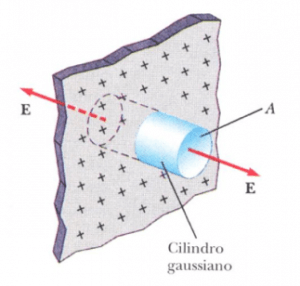
\includegraphics[scale=0.5]{Pictures/esempio4.png}
\end{figure}
Per il teorema di Gauss:
	\begin{displaymath}\begin{aligned}
		\epsilon_0 \cdot \Phi(\vec{E}) = q\\
        \epsilon_0 \cdot \int_S \vec{E} \cdot d\vec{A} = q\\
        \epsilon_0 \cdot (E\cdot A + E \cdot A) = q \cdot \sigma \cdot A\\
        2 \cdot \epsilon_0 \cdot E\cdot A = q = \sigma \cdot A\\
        E = \frac{\sigma}{2 \epsilon_0}
	\end{aligned}\end{displaymath}


\section{Energia elettrica}
\subsection{Energia potenziale elettrica}
L'energia potenziale è l'inverso del lavoro compiuto dalla forza per spostare $q_2$ dal punto $A$ al punto $B$.
	\begin{displaymath}\begin{aligned}
		\Delta U = - \int_A^B \vec{F} \cdot d\vec{s} = \\
        = - \int_A^B \vec{F} \cdot d\vec{r} = -\int_{r_A}^{r_B} k_e \cdot \frac{q_1 \cdot q_2}{r^2} dr =\\
        = k_e\cdot q_1 \cdot q_2 \cdot  \left(\frac{1}{r_B} - \frac{1}{r_A}\right)
	\end{aligned}\end{displaymath}

\subsection{Potenziale elettrico}
Sia $q_0$ una carica di prova in moto da $A$ a $B$, sotto l'azione di un campo elettrico $\vec{E}$:
	\begin{displaymath}
		\Delta V= \frac{\Delta U}{q_0} = \frac{-L_{AB}}{q_0} \qquad V = \frac{U}{q_0}
	\end{displaymath}

\subsection{Lavoro del campo elettrico}
Il lavoro compiuto dal campo elettrico per spostare una particella $q_0$ da $A$ a $B$:
\begin{displaymath}
	L_{AB} = q_0 \cdot (-\Delta V)		
\end{displaymath}


\subsection{La forza di Coulomb è conservativa}
Una forza è conservativa quando il lavoro da essa compiuto può essere scritto come una differenza di potenziale:
\begin{displaymath}\begin{aligned}
	L_{AB} = \int_A^B \vec{F} \cdot d\vec{r} = \int_A^B k_e \cdot \frac{q_1q_2}{r^2} \cdot \vec{u}_r \cdot d\vec{r} =\\
    = k_e \cdot q_1q_2 \cdot \int_A^B \frac{1}{r^2} = \left( k_e \frac{q_1q_2}{r_B}\right) - \left(k_e\frac{q_1q_2}{r_A}\right) = U(B) - U(A)
\end{aligned}\end{displaymath}
Questo risultato significa che:
\begin{itemize}
	\item{Il lavoro lungo un percorso chiuso è nullo.}
    \item{Il lavoro lungo uno spostamento dipende solo dal punto di partenza e dal punto di arrivo e non dal percorso seguito.}
\end{itemize}

\section{Dipolo elettrico}
Un dipolo elettrico è un sistema composto da due cariche uguali, di segno opposto, poste a distanza $d$ lungo un asse $u_x$.\\
\begin{figure}[h!]
	\centering
    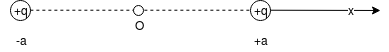
\includegraphics[scale=0.6]{Pictures/DipoloElettrico}
\end{figure}
Viene definito il \textbf{momento di dipolo} $\vec{p}$ come 
\begin{displaymath}
	\vec{p} = q \cdot d \cdot \vec{u}_x
\end{displaymath}

\subsection{Campo elettrico lungo l'asse del dipolo}
\begin{displaymath}\begin{aligned}
	\vec{E}_+ = k_e \cdot \frac{q}{(r_x - a)^2} \cdot \vec{i}\\
    \vec{E}_- = - k_e \cdot \frac{q}{(r_x + a)^2} \cdot \vec{i}\\\\
    \vec{E} = k_e \cdot \left(\frac{q}{(r_x - a)^2} - \frac{q}{(r_x^2 + a^2)^2} \right) \cdot \vec{i} = \\
    = k_e \cdot q \left( \frac{(r_x + a)^2 - (r_x - a)^2}{(r_x^2 + a^2)^2} \right) \cdot \vec{i} = \\
    = k_e \cdot q \frac{r_x^2 + a^2 + 2 r_x a - r_x^2 +2 r_x a - a^2}{(r_x^2 + a^2)^2} \cdot \vec{i} = 
    = k_e \cdot \frac{4 q r_x a}{(r_x^2 + a^2)^2} \cdot \vec{i}
\end{aligned}\end{displaymath}
Ricordando che $a = \frac{d}{2}$ e che $p = qd$:
\begin{displaymath}\begin{aligned}
	\vec{E} = k_e \cdot \frac{2p\cdot r_x}{(r_x^2 + \frac{d}{2}^2)^2} \cdot \vec{i}    
\end{aligned}\end{displaymath}
Ha senso, in applicazioni reali considerare $r_x >>> d$, cioè misurare il campo elettrico a distanze molto maggiori della distanza tra le cariche del dipolo.
\begin{displaymath}
\vec{E} = k_e \cdot \frac{2 p r_x}{r_x^4} \cdot \vec{i} = k_e \cdot \frac{2p}{r_x^3} \cdot \vec{i}
\end{displaymath}

\subsection{Potenziale elettrico lungo l'asse del dipolo}
Il potenziale generato da una carica a una distanza $r$ è dato da:
\begin{displaymath}
	V(r) = k_e \cdot \frac{q}{r}
\end{displaymath}
Perciò, il potenziale del dipolo a una distanza $r_x$ è dato da:
\begin{displaymath}\begin{aligned}
	V(r_x) = k_e \cdot \left( \frac{q}{r_x-a} - \frac{q}{r_x+a} \right) =\\ 
    k_e \cdot q \left( \frac{r_x + a - r_x + a}{r_x^2 -a^2} \right)=\\
    k_e \cdot q \cdot \frac{2a}{r_x^2-a^2}
\end{aligned}\end{displaymath}
Ricordando che $a = \frac{d}{2}$ e che $p = qd$:
\begin{displaymath}\begin{aligned}
	\vec{V} = k_e \cdot \frac{p}{r_x^2 - \frac{d}{2}^2}    
\end{aligned}\end{displaymath}
Ha senso, in applicazioni reali considerare $r_x >>> d$, cioè misurare il potenziale a distanze molto maggiori della distanza tra le cariche del dipolo.
\begin{displaymath}
	\vec{V} = k_e \cdot \frac{p}{r_x^2}
\end{displaymath}

\chapter{Magnetostatica}



\section{Forza di Lorentz}
Una carica in moto in un campo magnetico $\vec{B}$ è soggetta a una forza, detta \textbf{forza di Lorentz} $\vec{F}_B$ tale che:
\begin{displaymath}
	\vec{F}_B = q \vec{v} \times \vec{B}
\end{displaymath}
Poiché $\vec{F}_B$ è perpendicolare a $\vec{v}$, il modulo della velocità non può variare, ma solo la sua direzione.\\
Poiché $\vec{F}_B$ è perpendicolare allo spostamento, non può compiere lavoro sulla particella. Ciò significa che un campo magnetico uniforme non varia l'energia della particella.\\\\
Possiamo considerare tre casi:
\begin{itemize}
	\item{$\vec{v}$ parallelo a $\vec{B}$: il prodotto vettoriale è nullo e la particella non è soggetta a forza magnetica.}
    \item{$\vec{v}$ perpendicolare a $\vec{B}$: se $\vec{B}$ è costante, la particella si muove lungo una traiettoria circolare.}
    \item{Caso generale: la particella segue un moto ad elica lungo l'asse $\vec{u}_B$}
\end{itemize}

\subsection{Forza tra due fili paralleli percorsi da corrente}
\begin{figure}[h!]
	\centering
    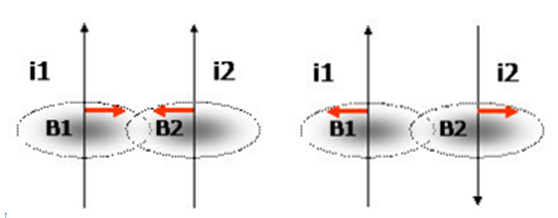
\includegraphics[scale=0.7]{Pictures/fili-paralleli-corrente.png}
\end{figure}
Un filo rettilineo percorso da corrente $I$ produce, a distanza $r$, un campo magnetico $\vec{B}$:
\begin{displaymath}
	\vec{B} = \mu_0 \cdot \frac{I}{2\pi r}
\end{displaymath}
Consideriamo la seguente configurazione: due fili, di lunghezza $L$, posti a distanza $D$ e percorsi, rispettivamente da una corrente $I_1$ e $I_2$.\\
Sul filo 1 agisce una forza $\vec{F}_{21}$ dovuta a $\vec{B}_2$, mentre sul filo 2 agisce una forza $\vec{F}_{12}$ dovuta a $\vec{B}_1$.\\
Tali forze, secondo la terza legge di Newton sono eguali in modulo e hanno direzioni opposte:
\begin{displaymath}\begin{aligned}
	\vec{F}_{12} = - \vec{F}_{21}
    F_{12} = F_{21} = B_2 \cdot I_1 \cdot d = B_1 \cdot I_2 \cdot d =\\ 
    \mu_0 \cdot \frac{I_1 \cdot I_2}{2 \pi d} \cdot L
\end{aligned}\end{displaymath}
La forza è attrattiva se i versi delle correnti sono concordi, mentre è repulsiva se sono discordi.

\section{Legge di Biot-Savart}
La legge di Biot-Savart permette di calcolare il campo magnetico prodotto da un filo percorso da corrente:
\begin{displaymath}
	\vec{B} = \frac{\mu_0}{4\pi} \cdot \int \frac{i \cdot d\vec{s} \times \vec{r}}{r^3}
\end{displaymath}

\subsection{Tratto di filo rettilineo}
Calcoliamo il campo magnetico generato da un filo di lungezza $L$ percorso da corrente $I$, a una distanza $r$:
\begin{displaymath}
	\vec{B} = \mu_0 \cdot  \frac{I}{4 \pi \cdot r} \cdot  \frac{L}{\sqrt{\frac{L}{4} + r^2}}
\end{displaymath}
Se il filo ha lunghezza infinita o è molto più lungo rispetto alla distanza a cui misuriamo il campo elettrico ($L>>>d$)
\begin{displaymath}
	\vec{B}=\mu_0 \cdot \frac{I}{2 \pi r}
\end{displaymath}

\subsection{Spira circolare}
Consideriamo una spira circolare di raggio $R$ percorsa da una corrente $I$.\\
Calcoliamo il campo magnetico $\vec{B}$ che essa genera in un punto $P$ posto sull'asse perpendicolare alla spira e passante per il suo centro.\\
$P$ si trova a una distanza $z$ dal centro della spira.
\begin{figure}[h!]
	\centering
	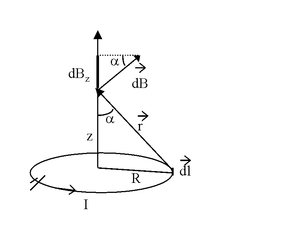
\includegraphics[]{Pictures/biotSavart.png}
\end{figure}
Scomponiamo $d\vec{B}$ in due componenti:
\begin{itemize}
\item{$dB_z$ lungo l'asse $z$}
\item{$dB_p$ perpendicolare a $dB_z$: per ragioni di simmetria, la somma di tutti i componenti $dB_p$ è nulla}
\end{itemize}
Usiamo la legge di Biot-Savart per calcolare $dBz$:
\begin{displaymath}\begin{aligned}
	dB_z = \mu_0 \cdot \frac{I \cdot \cos{\alpha} \cdot ds}{4\pi \cdot r^2}\\
    r^2 = R^2 + z^2 \qquad \cos{\alpha} = \frac{R}{r} = \frac{R}{\sqrt{R^2 + z^2}}\\
    dB_z = \mu_0 \cdot \frac{I \cdot R}{4\pi \cdot (R^2 + z^2)^\frac{3}{2}}\\
\end{aligned}\end{displaymath}

Il campo magnetico totale $B$ è pari a:
\begin{displaymath}\begin{aligned}
	\vec{B} = \int dB_z \cdot \vec{k} =  \mu_0 \cdot \frac{I \cdot R}{4\pi \cdot (R^2 + z^2)^\frac{3}{2}} \cdot \int dS \cdot \vec{k} = \\
    = \mu_0 \cdot \frac{I \cdot R}{4\pi \cdot (R^2 + z^2)^\frac{3}{2}} \cdot 2 \pi \cdot R \cdot \vec{k} = \\
    =\mu_0 \cdot \frac{I \cdot R^2}{2 \cdot (R^2 + z^2)^\frac{3}{2}} \cdot \vec{k}
\end{aligned}\end{displaymath}

Nel centro della spira ($r=R$):
\begin{displaymath}\begin{aligned}
	\vec{B} = \int dB_z \cdot \vec{k} =  \mu_0 \cdot \frac{I \cdot R}{4\pi \cdot (R^2 + z^2)^\frac{3}{2}} \cdot \int dS \cdot \vec{k} = \\
    = \mu_0 \cdot \frac{I}{2R} \vec{k}
\end{aligned}\end{displaymath}

\section{Legge di Ampére}
La legge di Ampére ci permette di calcolare la circuitazione del campo magnetico lungo una linea chiusa
\begin{displaymath}
	\oint \vec{B} \cdot d\vec{s} = \mu_0 \cdot I
\end{displaymath}

\subsection{Solenoide ideale}
Un solenoide è caratterizzato da una corrente $I$ che scorre in un filo avvolto a spirale $n$ volte per unità di lunghezza intorno ad un cilindro di raggio $a$ e lunghezza $L$.\\
Se $a <<< L$, il campo magnetico $\vec{B}$ è, in prima approssimazione, contenuto all'interno del solenoide, in direzione assiale, con intensità costante. In queste condizioni (ideali),  
\begin{figure}[h!]
	\centering
	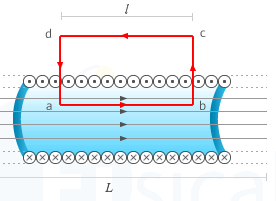
\includegraphics[scale=3]{Pictures/solenoide-ampere.png}
\end{figure}
\begin{displaymath}\begin{aligned}
	\oint \vec{B} \cdot d\vec{s} = \int_A^B \vec{B} \cdot d\vec{s} + \int_B^C \vec{B} \cdot d\vec{s} + \int_C^D \vec{B} \cdot d\vec{s} + \int_D^A \vec{B} \cdot d\vec{s} + 
\end{aligned}\end{displaymath}
Il secondo e il quarto integrale sono nulli, in quanto o il campo $\vec{B}$ è parallelo al cammino di integrazione (punti interni) o è nullo (punti esterni).\\
Il terzo integrale è nullo perché abbiamo assunto $\vec{B}$ nullo all'esterno del solenoide.
\begin{displaymath}
	\oint \vec{B} \cdot d\vec{s} = \int_A^B \vec{B} \cdot d\vec{s} = B \cdot l\\
\end{displaymath}
Utilizzando la legg e di Ampére:
\begin{displaymath}
	B = \mu_0 \cdot \frac{I}{L}
\end{displaymath}

\section{Legge di Faraday-Lenz}
Secondo la legge di Faraday-Lenz, a una variazione del flusso del campo magnetico corrisponde una f.e.m. autoindotta che si oppone a tale variazione.
\begin{displaymath}
	- \frac{d\Phi_S (\vec{B})}{dt} = \epsilon_{indotta}
\end{displaymath}

\subsection{Relazione con induttanza}
Consideriamo un solenoide, in cui $S$ è la superficie della sezione della spira, l'induttanza è $L$ e la corrente che lo percorre $i(t)$. 
\begin{displaymath}\begin{aligned}
	\Phi_S (\vec{B}) = L \cdot i(t) = \oint \vec{B} \cdot \vec{n}\\
    \frac{d\Phi_S (\vec{B})}{dt} = L \cdot \frac{di}{dt}
\end{aligned}\end{displaymath}
Utilizzando la legge di Ampére
\begin{displaymath}
	\epsilon_{indotta} = -L \cdot \frac{di}{dt}
\end{displaymath}
\chapter{Circuiti}

\section{Corrente elettrica}
La corrente elettrica $i$ è definita come la quantità di carica che nell'unità di tempo attraversa un elemento di area entro un conduttore.\\
Il verso della corrente è quello in cui si muovono le cariche positive, anche quando, nella realtà i portatori di carica dovessero essere negativi.

\subsection{Leggi di Kirchhoff}
\textbf{Prima legge Kirchhoff (ai nodi)}: \textit{In qualunque nodo di un circuito elettrico la corrente totale entrante è uguale alla corrente totale uscente.}\\
\textbf{Seconda legge Kirchhoff (alle maglie)}: \textit{la somma algebrica di tutte le differnze di potenziale di una maglia è zero.}

\section{Analisi dei circuiti}
Solitamente lo scopo dell'analisi di un circuito consiste nel trovare la corrente in modulo e verso, dati i valori di f.e.m. e resistenza del circuito.\\
Attribuire arbitrariamente il segno della corrente: nella maggior parte dei casi siamo in grado di sceglierlo correttamente (per esempio sfruttando i generatori di corrente, in quanto la corrente va dal polo negativo a quello positivo), ma se dovessimo sceglierlo in maniera errata, ciò verrà segnalato dal segno negativo della corrente che otterremo come risultato.\\
Partendo da un qualunque punto fissato arbitrariamente, percorrere un giro completo della maglia sommando algebricamente le differenze di potenziale che via via si incontrano ai capi di tutti gli elementi, applicando la legge di Kirchhoff alle maglie.
\begin{esempio}
	Consideriamo il seguente circuito:
	\begin{figure}[h!]
		\centering
		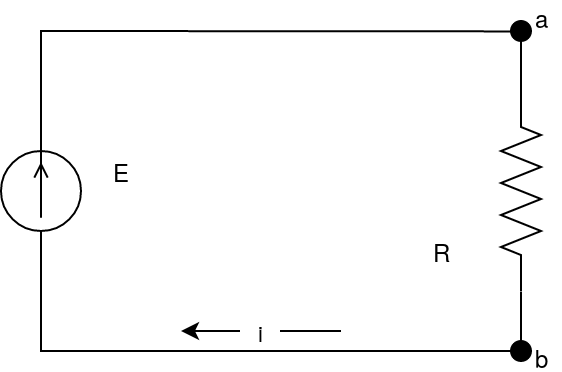
\includegraphics[scale=0.4]{Pictures/circuito}
		\caption{Circuito}
	\end{figure}
	Partendo dal punto $a$, in cui il potenziale ha valore $V_a$, procediamo in senso orario: incontriamo dapprima il resistore, attraverso il quale il potenziale cade di $\Delta V_R = i\cdot R$, cosicché il potenziale in $b$ risulta $V_b = V_a - i\cdot R$.\\
	Proseguendo, incontriamo la batteria, ove entriamo dal polo negativo, per cui il potenziale cresce di una quantità pari alla f.e.m. $E$.\\
	Possiamo quindi scrivere
	\begin{displaymath}
		V_a = V_b + E = V_a - i \cdot R + E
	\end{displaymath}
	Sfruttando la legge di Kirchhoff alle maglie:
	\begin{displaymath}\begin{aligned}
		E - i \cdot R = 0\\
		i = \frac{E}{R}
	\end{aligned}\end{displaymath}
\end{esempio}

\subsection{Differenza di potenziale nei circuiti}
Per determinare la differenza di potenziale tra due punti qualsiasi di un circuito, si parte da un punto e ci si sposta lungo il circuito verso l'altro punto, sommando algebricamente le variazioni di potenziale incontrate.\\
Questa somma algebrica è la differenza di potenziale tra i punti.\\\\
Si può seguire un \textbf{qualunque} cammino tra i due punti lungo il circuito ottenendo lo stesso valore di differenza di potenziale, dato che un aspetto fondamentale del concetto di potenziale è l'indipendenza dal cammino.

\subsection{Forza elettromotrice}
Per spostare le cariche nei circuiti elettrici è generalmente necessaria una sorgente esterna di energia. Il circuito deve quindi contenere un dispositivo che mantenga una differenza di potenziale tra due punti.\\
Un qualunque dispositivo che svolga questo compito in un circuito elettrico è detto sorgente di \textbf{forza elettromotrice}. Può essere utile considerare un generatore di f.e.m. come un meccanismo che crea un'elevazione di potenziale, vi \textit{innalza} le cariche, da cui esse \textit{cadono} poi verso \textit{valle} attraverso il resto del circuito.\\\\

\subsection*{Elementi circuitali in parallelo}
Due o più elementi circuitali collegati in parallelo godono delle seguenti proprietà:
\begin{itemize}
\item{Ci si può spostare da un capo all'altro della configurazione attraversando un solo elemento.}
\item{Su ciascun elemento appare la stessa differenza di potenziale.}
\item{La corrente si suddivide tra i vari elementi.}
\end{itemize}

\subsection*{Elementi circuitali in serie}
Due o più elementi circuitali collegati in serie si godono delle seguenti proprietà:
\begin{itemize}
\item{Per passare da un capo all'altro della configurazione è necessario attraversare in successione tutti gli elementi.}
\item{La differenza di potenziale applicata agli estremi è pari alla somma delle differenze di potenziali su ciascun elemento.}
\item{Tutti gli elementi sono percorsi dalla stessa corrente.}
\end{itemize}

\section{Resistori}

\subsection{Resistori collegati in parallelo}
\begin{figure}[h!]
	\centering
    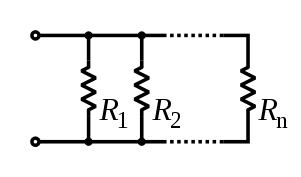
\includegraphics[scale=0.5]{Pictures/resistori-parallelo}
\end{figure}
Calcoliamo la resistenza equivalente di due resistori collegati in parallelo:
\begin{displaymath}\begin{aligned}
	i_1 = \frac{\Delta V}{R_1} \qquad i_2 = \frac{\Delta V}{R_2} \qquad i = i_1 + i_2 = \frac{\Delta V}{R}\\
    \frac{\Delta V}{R} = \frac{\Delta V}{R_1} + \frac{\Delta V}{R_2}\\
    \frac{1}{R} = \frac{1}{R_1} + \frac{1}{R_2}\\
\end{aligned}\end{displaymath}
Possiamo dimostrare, per induzione, che per $n$ resistori vale:
\begin{displaymath}
	\frac{1}{R} = \sum_{i=1}^n \frac{1}{R_i}
\end{displaymath}

\subsection{Resistori collegati in serie}
\begin{figure}[h!]
	\centering
    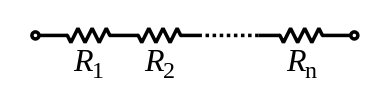
\includegraphics[scale=0.5]{Pictures/resistori-serie}
\end{figure}
Calcoliamo la resistenza equivalente $R$ di due resistori collegati in serie:
\begin{displaymath}\begin{aligned}
	\Delta V_1 = i \cdot R_1 \qquad \Delta V_2 = i \cdot R_2 \qquad \Delta V = \Delta V_1 + \Delta V_2 = i \cdot R \\ 
    i \cdot R = i \cdot R_1 + i\cdot R_2\\
    R = R_1 + R_2
\end{aligned}\end{displaymath}

Possiamo dimostrare, per induzione, che per $n$ resistori vale:
\begin{displaymath}
	R = \sum_{i=1}^n R_i
\end{displaymath}

\section{Condensatori}
Un condensatore piano è un sistema costituito da due superfici piane di materiale conduttore, aventi superficie $S$, poste a distanza $d$, in modo da costituire due piani paralleli.\\
Una superficie è caricata positivamente, l'altra negativamente.

\subsection{Campo elettrico all'interno di un condensatore}
All'interno del condensatore è presente un campo elettrico uniforme. Vediamo come calcolarlo.\\\\
Per il teorema di Gauss, una superficie piana carica genera un campo elettrico pari a:
\begin{displaymath}
	E = \frac{\sigma}{2 \cdot \epsilon_0}
\end{displaymath}
Poiché in un condensatore abbiamo due piani carichi sarà:
\begin{displaymath}
	E = 2 \cdot \frac{\sigma}{2 \cdot \epsilon_0} = \frac{\sigma}{\epsilon_0}
\end{displaymath}
Poiché $\sigma = \frac{Q}{S}$ possiamo scrivere:
\begin{displaymath}
	E = \frac{Q}{S \cdot \epsilon_0}
\end{displaymath}
Ricordiamo che il vettore campo elettrico è entrante per la lastra con carica negativa, e uscente per la piastra con carica positiva.\\
Possiamo dedurre che all’esterno delle due lastre il contributo al campo elettrico di ciascuna di esse fa si che il campo elettrico totale sia nullo; all’interno di esse, invece, il campo elettrico è doppio rispetto a quello generato da ogni singola armatura.

\subsection{Differenza di potenziale sulle armature del condensatore}
Utilizziamo la definizione di energia potenziale (in cui il punto A rappresenta una delle armature e il punto B rappresenta l'altra):
\begin{displaymath}
	\Delta V = \int_A^B \vec{E} \cdot d\vec{s}
\end{displaymath}
Poiché i versori che indicano la direzione di $\vec{E}$ e $d\vec{S}$ sono paralleli, il loro prodotto scalare è pari a 1, quindi:
\begin{displaymath}
	\Delta V = \frac{Q}{S \cdot \epsilon_0} \cdot d
\end{displaymath}

\subsection{Capacità di un condensatore piano}
La capacità di un condensatore è il rapporto tra la carica che può immagazzinare e la differenza di potenziale sulle armature.\\
Si tratta di una costante che dipende soltanto dalle caratteristiche fisiche e geometriche del condensatore.
\begin{displaymath}
	C = \frac{Q}{\Delta V} = Q \cdot \frac{S \cdot \epsilon_0}{Q \cdot d} = \frac{S \cdot \epsilon_0}{d} 
\end{displaymath}

\subsection{Cosa accade all'esterno del condensatore}
Come abbiamo detto nel paragrafo 4.2.1, il campo elettrico all'esterno del condensatore è nullo. Ciò implica che sia nullo anche il potenziale.

\subsection{Carica e scarica del condensatore}
\subsubsection{Processo di carica}
La carica si accumula sulle armature del condensatore quando viene applicata una differenza di potenziale $\Delta V = \epsilon$
\begin{displaymath}\begin{aligned}
	Q(t) = Q_{MAX} \cdot (1- e^{\frac{-t}{RC}})\\
    Q(t) = C \cdot \Delta V \cdot (1- e^{\frac{-t}{RC}})
\end{aligned}\end{displaymath}
\begin{itemize}
	\item{$t < 0$: condensatore scarico}
    \item{$t \rightarrow 0$: condensatore in carica 
    	\begin{displaymath}\begin{aligned}
            Q(t) = Q_{MAX} \cdot (1- e^{\frac{-t}{RC}}) = 
            Q_{MAX} \cdot (1- e^{\frac{-0}{RC}}) = 
            Q_{MAX} \cdot (1- 1) = 0
    	\end{aligned}\end{displaymath}}
    \item{$t \rightarrow \infty$: condensatore carico a regime
      \begin{displaymath}\begin{aligned}
              \Delta V = \epsilon\\
              Q(t) = Q_{MAX} (1- e^{\frac{-\infty}{RC}}) = 
              Q_{MAX} = C \cdot \epsilon
          \end{aligned}\end{displaymath}}
\end{itemize}

\subsubsection{Processo di scarica}
La carica accumulata sulle armature viene rilasciata, generando una $\Delta V = \epsilon$.
\begin{displaymath}\begin{aligned}
	Q(t) = Q_{MAX} \cdot (e^{\frac{-t}{RC}})\\
    Q(t) = C \cdot \Delta V \cdot (e^{\frac{-t}{RC}})
\end{aligned}\end{displaymath}
\begin{itemize}
	\item{$t < 0$: condensatore carico
    	\begin{displaymath}\begin{aligned}
    		Q(t) = Q_{MAX} (e^{\frac{-0}{RC}}) = Q_{MAX} = C \cdot \epsilon
    	\end{aligned}\end{displaymath}}
    \item{$t \rightarrow 0$: condensatore inizia a scaricarsi 
    	\begin{displaymath}\begin{aligned}
            Q(t) = Q_{MAX} \cdot (e^{\frac{-t}{RC}})\\
    Q(t) = Q_{MAX} \cdot (e^{\frac{-0}{RC}}) = Q_{MAX} = C \cdot \epsilon
    	\end{aligned}\end{displaymath}
        Il condensatore si comporta come un generatore avente una fem pari a 
        \begin{displaymath}
        	\epsilon = \frac{Q_{MAX}}{C}
        \end{displaymath}}
    \item{$t \rightarrow \infty$: condensatore scarico
      	\begin{displaymath}\begin{aligned}
        	Q(t) = Q_{MAX} \cdot (e^{\frac{-\infty}{RC}}) = 0
         \end{aligned}\end{displaymath}}
\end{itemize}

\subsection{Condensatori collegati in parallelo}
\begin{figure}
	\centering
    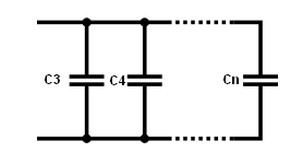
\includegraphics[scale = 0.7]{Pictures/condensatori-parallelo}
\end{figure}
Calcoliamo la capacità equivalente $C$ di due condensatori collegati in serie:
\begin{displaymath}\begin{aligned}
	q_1 = C_1 \cdot \Delta V \qquad q_2 = C_2 \cdot \Delta V \qquad q = q_1 + q_2 = C \cdot \Delta V\\
    C \Delta V = C_1 \Delta V + C_2 \Delta V\\
    C = C_1 + C_2
\end{aligned}\end{displaymath}
Possiamo dimostrare, per induzione, che per $n$ condensatori vale:
\begin{displaymath}
	C = \sum_{i=1}^n C_i
\end{displaymath}

\subsection{Condensatori collegati in serie}
\begin{figure}[h!]
	\centering
    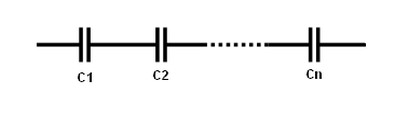
\includegraphics[scale = 0.8]{Pictures/condensatori-serie}
\end{figure}
Calcoliamo la capacità equivalente di due condensatori collegati in parallelo:
\begin{displaymath}\begin{aligned}
	\Delta V_1 = \frac{q}{C_1} \qquad \Delta V_2 = \frac{q}{C_2} \qquad
    \Delta V = \Delta V_1 + \Delta V_2 = \frac{q}{C}\\
    \frac{q}{C} = \frac{q}{C_1} + \frac{q}{C_2}\\
    \frac{1}{C} = \frac{1}{C_1} + \frac{1}{C_2}
\end{aligned}\end{displaymath}

Possiamo dimostrare, per induzione, che per $n$ resistori vale:
\begin{displaymath}
	\frac{1}{C} = \sum_{i=1}^n \frac{1}{C_i}
\end{displaymath}

\section{Induttori}
L'induttore è quell'elemento circuitale che immagazzina energia nel campo magnetico generato dalle sue spire percorse da corrente, proprio come il condensatore accumula energia nel campo elettrico tra le sue armature cariche.\\
Un induttore è caratterizzato da un'\textbf{induttanza}, una grandezza che dipende dalle proprietà geometriche.\\
L'induttanza $L$ è definita come la costante di proporzionalità tra la f.e.m. indotta e la derivata temporale della corrente: $$\epsilon_L = L \cdot \frac{di}{dt}$$
Il verso della f.e.m. indotta è tale da opporsi alla variazione di corrente.

\subsection{Induttori nei circuiti}
All'istante iniziale l'induttore si comporta come una resistenza di valore infinito, che pian piano si riduce a zero quando la corrente raggiunge il suo valore stazionario.\\
%\includepdf[pages={1-60}]{temi-esame.pdf}
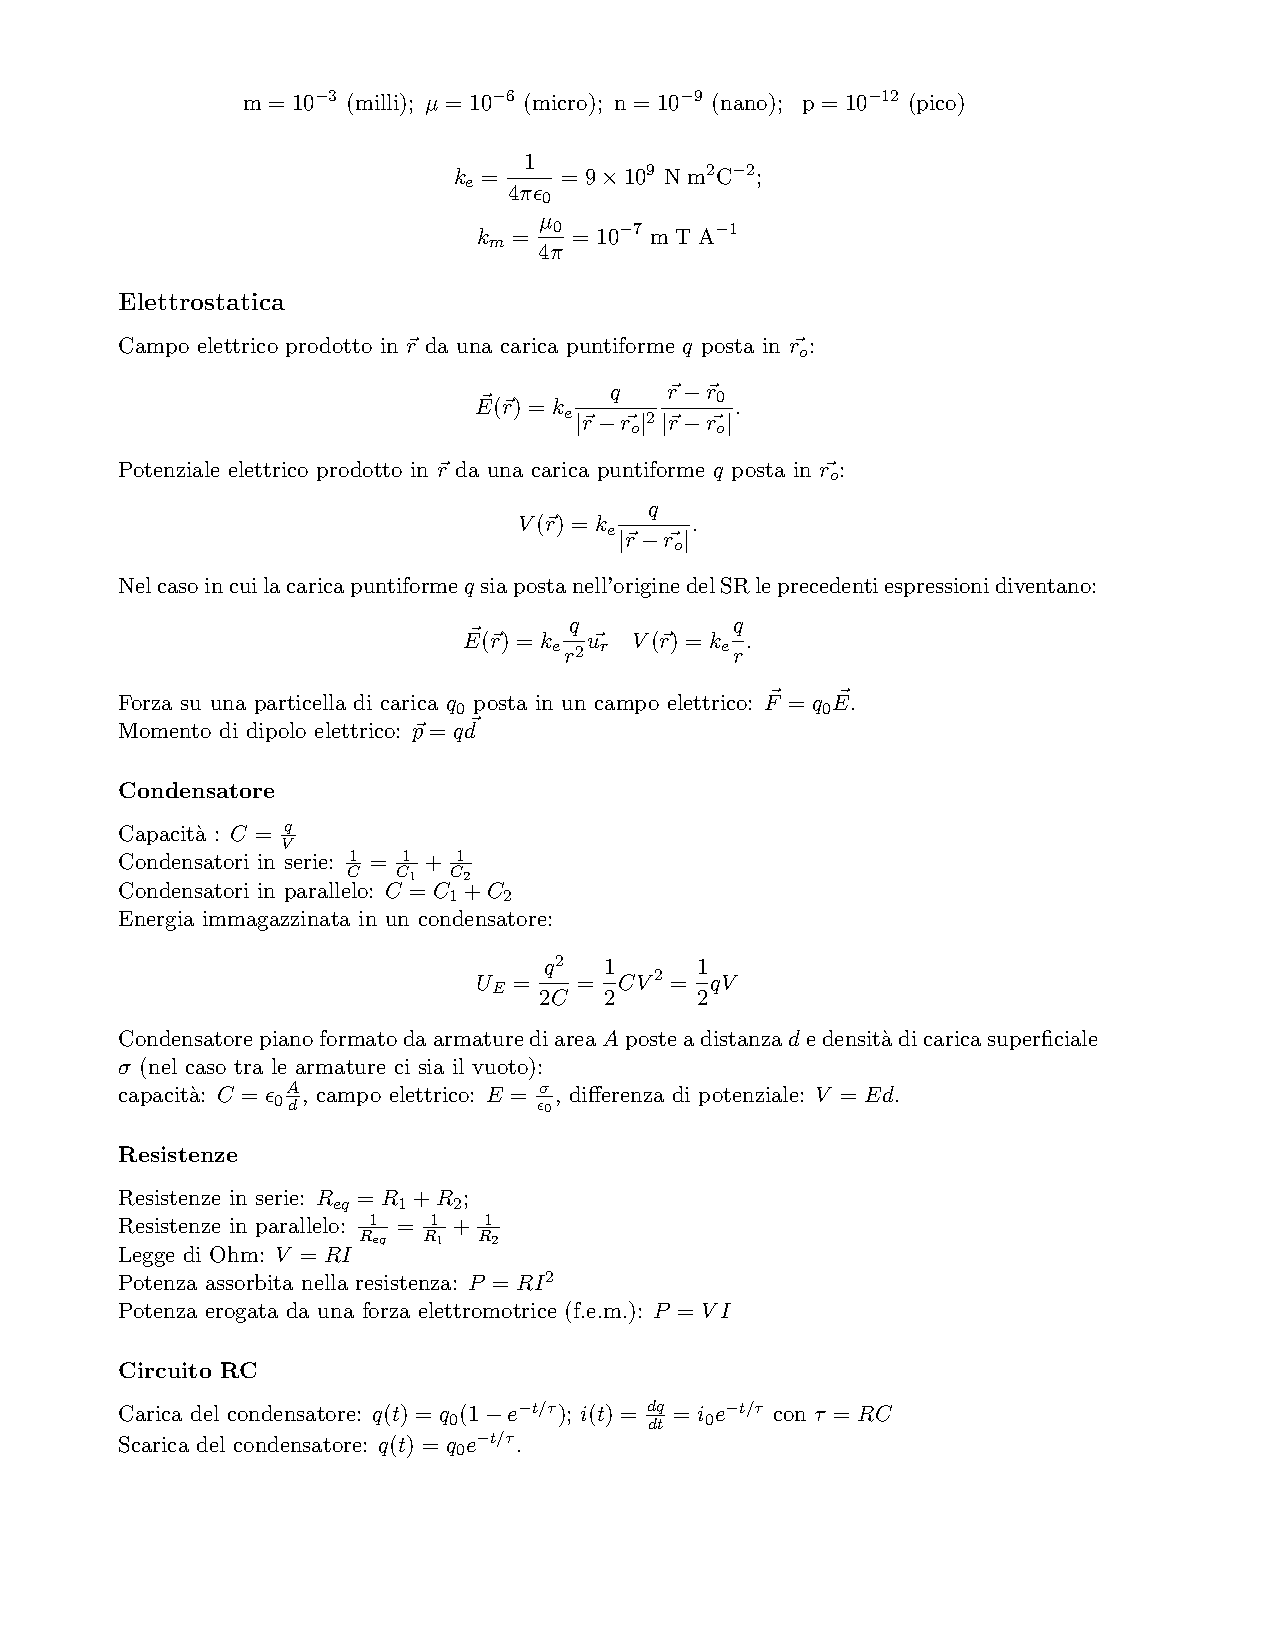
\includepdf[pages={1-2}]{formulario.pdf}

\end{document}
